\documentclass[12pt]{article}

 \usepackage{graphics}
\usepackage{enumitem}

\usepackage{geometry}
  \geometry{
    a4paper,
    total={6in, 9in},
    top=20mm,
  }

\usepackage{graphicx}
\graphicspath{ {./img/} }

\usepackage{array}
\newcolumntype{P}[1]{>{\centering\arraybackslash}p{#1}}

\usepackage{multirow}
\usepackage{subcaption}
\usepackage{hyperref}

\usepackage{pgfplots}
\pgfplotsset{width=5in,compat=1.9}

\title{Tema 1}
\author{Renghiuc Bianca Elena, Chichirău Claudiu-Constantin 2A2}
\date{04.11.2022}

\begin{document}
\maketitle

\section{Execi\c{t}iul 1}
  \begin{itemize}
    \item[a)] Fiecare component\u{a} conex\u{a} din graful G=(V,E) reprezint\u{a} mul\c{t}imea tuturor tripletelor ($start_i$, $station_i$, $end_i$)  \^{i}n care $' station_i '$ este aceea\c{s}i pentru toate tripletele, iar $(start_i, end_i) \bigcap (start_j, end_j) \neq \emptyset$, oricare ar fi $0 \leq i \leq k-1$, $0 \leq j \leq k-1$. 
 
    Pentru fiecare sta\c{t}ie exist\u{a} cel pu\c{t}in o component\u{a} conex\u{a}. De exemplu dac\u{a} un numar de tramvaie x se intersecteaz\u{a}  \^{i}ntr-un interval de timp x', \^{i}n aceea\c{s}i sta\c{t}ie z, ele formeaz\u{a} o component\u{a} conex\u{a}. Un alt num\u{a}r de tramvaie y se pot intersecta \^{i}ntr-un interval de timp y', \^{i}n aceea\c{s}i sta\c{t}ie z, form\^{a}nd o alt\u{a} component\u{a} conex\u{a}, \^{i}n care $x \neq x', y \neq y'$.
    
    $\Longrightarrow nr.componente.conexe \geq nr.stații.tramvai$
    \item[b)] 
    Ca să aflăm numărul maxim de tramvaie ce se pot afla simulta într-o aceeași stație $i$ ne ajutăm de subpunctul a). în
	care am arătat că fiecărei stații de tramvai îi corespunde cel puțin o componentă conexă. 

	    Într-o componentă conexă două triplete ($start_i$, $station_i$, $end_i$) și ($start_j$, $station_i$, $end_j$) sunt adiacte $\iff (start_i$, $end_i$) $\bigcap$ ($start_j$, $end_j) \neq \emptyset$ (timpul la care tramvaiele ajung în stație și/sau pleacă 
	din stație au o componentă în comun $\Longrightarrow$ se află pentru un moment simultan în aceeași stație de tramvai). 
	
Astfel, dacă $n$ tramvaie se află în același interval de timp într-o $statie_i$, ele vor forma o componentă conexă cu $n$ noduri. Această componentă conexă este un graf complet $K_n$ cu $n$ noduri deoarece fiecare tramvai $i$ ($i \in \{ 1, ...,n \} )$ va fi adiacent cu oricare alt tramvai $j$ ($j \in \{1, ...,n \} \backslash \{ i \}) $ din aceeași componentă, aflându-se în același interval de timp în $statia_i$. 

Așadar, fiecare componentă conexă va reprezenta un graf complet ceea ce înseamnă că numărul maxim de tramvaie ce se pot afla simultan într-o aceeași $stație_i$ reprezintă cel mai mare graf complet $K_n$ cu $n$ noduri, numit și $n-clică$ = $ \omega (G)$.

  
  
    \item[c)]
    
    Presupunem că graful G=(V,E) ar putea conține circuite induse de lungime $ \geq 4 $.  
    
    Alegem un circuit cu $x$ noduri, $x \geq 4 $,  și vrem să aflăm dacă acesta este indus sau nu. Știm că un circuit indus cu număr $par$ de noduri are o $2-colorare$, în timp ce un circuit indus cu număr $impar$ de noduri are o $3-colorare$.  Componentele conexe din graful G=(V,E) sunt grafuri complete $K_n$, deci un subgraf cu $y$ noduri, $ y \leq x $, al unei astfel de componente va fi la rândul său graf complet. Totodată știm că orice graf complet $K_n$ cu $n$ noduri are o $n-colorare$ deoarece fiecare pereche de noduri distincte este conectată printr-o muchie unică. În acest caz orice circuit am alege de lungime $\geq 4 $ are o $n-colorare$, unde $n \geq 4$, ceea ce nu respectă cerința circuitului indus. 
    
    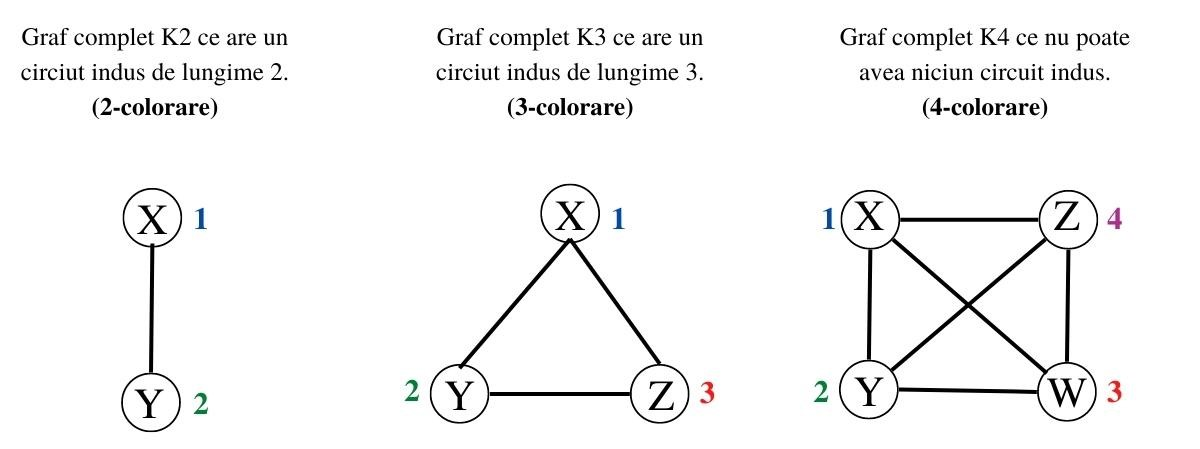
\includegraphics[scale=0.48]{Tema_1_c.jpg}
    
    Ajungem astfel la o contradicție $\Longrightarrow$ graful G=(V,E) nu poate avea circuite induse de lungime n, unde $ n \geq 4 $.

    
    \item[d)]
    Structura de date necesară implementării în $O ( \, 1 ) \,$ a operației $ ( \, * ) \,$ este reprezentată de o listă de adiacență. Pentru a stoca  valorile $visitedNeighbors [ \, u ] \,$ vom avea nevoie de o coada. În acest caz a treia instructiune $”for”$ din algoritmul prezentat va fi parcursă doar de $d_G(u)$ ori (pentru toți $u \in V$, fapt rezultat din structura de date necesară implementării operației $ ( \, * ) \,$ prezentată mai sus).
    
    Știind că a treia instrucțiune $”for”$ este parcursă de suma gradelor a tuturor nodurilor $u \in V$ ori putem spune că complexitatea întregului algoritm va fi $O ( \, n + \Sigma_{u \in V}d_G(u))$ = $O ( \, n + 2m) $ = $O(n+m)$, unde $n=|V|$ iar $m=|E|$.
    
    
    
    \item[e)]
    Funcționarul primăriei a demonstrat că oricare ar fi o componentă conexă cu n noduri din $G_i = [ \, \{ x_i, x_{i+1}, ..., x_n 	\} ] \,$, $ 1 \leg i \leq n$ ce reprezintă $N_G_i(x_i)$ în graful G aceasta este o n-clică. Știind că algoritmul dat determină valoarea maximă a lui $d_G(x_i)$, tot ceea ce trebuie să facem pentru a determina valoarea lui $ \omega (G)$ este să parcurgem toate componentele conexe și să determinăm care dintre ele are cele mai multe noduri.  

    \end{itemize}



\section{Exerci\c{t}iul 2}
\begin{itemize}
    \item[a)] 
Pentru a demonstra că proprietatea P este adevărată pentru grafuri 
complete, alegem graful complet $K_n$=(V,E) și două orientări aciclice 
$K_n'$=(V, A') și $K_n''$=(V, A'').

Aplicăm algoritmul pentru a afla o ordonare topologică a orientării aciclice $K_n'$ și vom obține ordonarea $x_1$, $x_2$, ..., $x_n$. Pentru ca digraful $K_n'$ să nu-și schimbe proprietate de orientare aciclică prin $reverse$ de un arc trebuie să alegem arcul $\vec{uv}$ sau $\vec{vu}$ astfel încât nodurile $u$ și $v$ sunt plasate consecutiv în ordonarea topologică și arcul aparține mulțimii $A'\backslash A''$.
Arcele care se formează din nodurile consecutive ale ordonării topologice vor forma un drum, astfel nodul de unde începe drumul va avea gradul interior 0. Adăugăm arce păstrând proprietatea de digraf aciclic până ajungem la un graf complet (demonstrație la punctul c).

Astfel există un singur digraf ce poate conține arcele formate din nodurile consecutive ale ordonării topologice, așa că în A'' trebuie să se inverseze măcar unul din aceste arce. Deci arcul $\vec{uv}$ sau $\vec{vu}$ prezentat anterior va aparține sigur mulțimii $A'\backslash A''$.


$\Longrightarrow$ e $\in$  $A'\backslash A''$ astfel încât $reverse$($K_n'$, e) este tot o orientare aciclică a lui $K_n$.

    
    \item[b)] 
    Pentru a demonstra că orice $\vec{K_n'}$ poate fi transformat într-un $\vec{K_n''}$ prin aplicări repetate ale operației $reverse$, ne folosim de principiul inducției matematice.

	Notăm cu P(k): $K_n$=(V,E), $\vec{K_n'}$=(V, A') și $\vec{K_n''}$=(V, A'') două ordonări aciclice ale lui $K_n$, iar $k = | A'$ $\backslash$ $A'' |$.
	
	$Etapa$ $de$ $verificare$: \\
	k=1 $\Longrightarrow$ P(1): Fie graful $K_n$=(V,E) de mai jos, $\vec{K_n'}$=(V, A') și $\vec{K_n''}$=(V, A'') două ordonări aciclice ale lui $K_n$, unde  $k = | A'$ $\backslash$ $A'' | = 1$.

    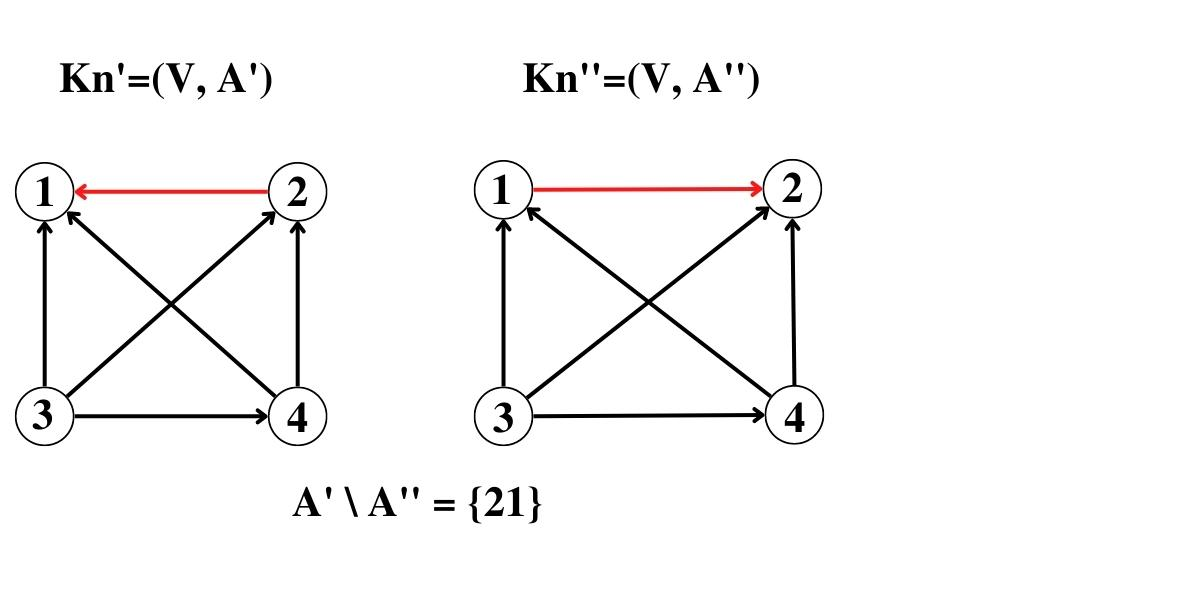
\includegraphics[scale=0.5]{Tema_2_b.jpg}

	Observăm că mulțimea $| A'$ $\backslash$ $A'' | = e = \{ 21 \} $. Deci, tot ceea ce trebuie să facem pentru a ajunge la ordonarea aciclică $\vec{K_n''}$ din $\vec{K_n'}$ este să aplicam $reverse(\vec{K_n'}, e)$ și astfel obținem ordonarea aciclică $\vec{K_n''}$ $\Longrightarrow$ P(1) Adevărat. \\

	$Etapa$ $de$ $demonstrație$: \\
	Presupunem că propoziția P(k): $K_n$=(V,E), $\vec{K_n'}$=(V, A') și $\vec{K_n''}$=(V, A'') două ordonări aciclice ale lui $K_n$, unde $k = | A'$ $\backslash$ $A'' |$ este adevărată. \\

	$Demonstrăm$ $că$ $propoziția$ $P(k+1)$ $este$ $adevărată$: \\
	P(k+1): $K_n$=(V,E), $\vec{K_n'}$=(V, E') și $\vec{K_n''}$=(V, E'') două ordonări aciclice ale lui $K_n$, unde $k+1 = | E'$ $\backslash$ $E'' |$. 

 
    $ A' \subset E', A'' \subset E''$, iar $k = | A'$ $\backslash$ $A'' |$.

$| E' \backslash E'' | = | (A' \cup e_1) \backslash (A'' \cup e_2) | $ , unde $e_1$ = $reverse(e_2)$, deci $e_1$ $\neq$ $e_2$.

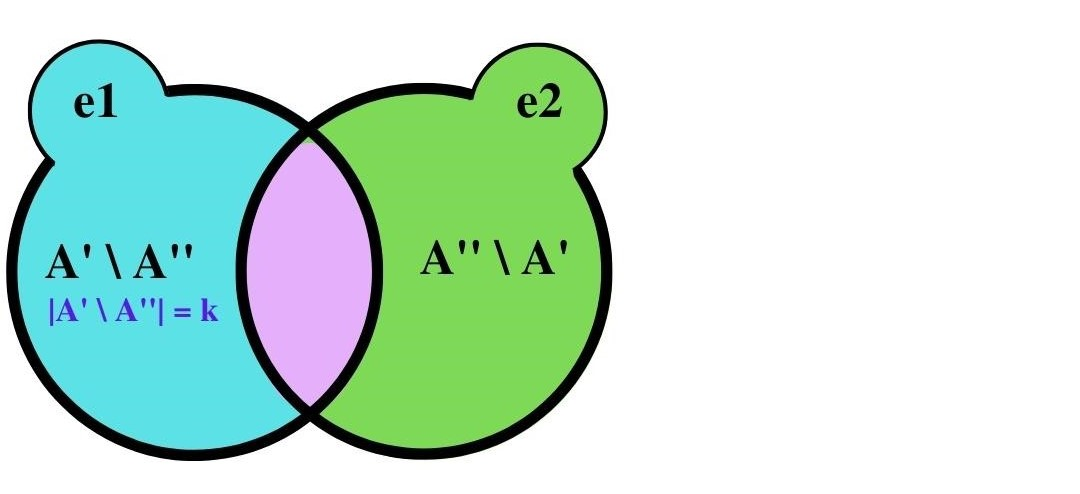
\includegraphics[scale=0.4]{Tema_2_b'.jpg}

 Se observă în desenul de mai sus că mulțimea $| A' \backslash A'' |$ are $k$ elemente. Dacă reunim la mulțimea A' pe $e_1$ $\notin$ $A''$ și la $A''$ reunim pe $e_2$ $\notin$ $A'$, observăm că vom obține aceleași $k$ elemente din $A' \backslash A''$ plus elementul $e_1$ (deci $k+1$ elemente) atunci când vom face scăderea dintre $ (A' \cup e_1) \backslash (A'' \cup e_2) $. 

	$ \Longrightarrow |E'-E''| = k+1 $
		
Așadar, P(k+1) este adevărată $ \Longrightarrow $ P(k) este adevărat $ \Longrightarrow $ $\vec{K_n'}$ poate fi transformat în $\vec{K_n''}$ prin aplicări repetate ale operației reverse.
    \item[c)]

Un digraf este aciclic dacă și numai dacă admite o ordonare topologică, deci orice orientare aciclică, $\vec{G}$ $=(V,A)$ , a unui graf $G=(V,E)$ are o ordonare topologică.
Ceea ce insemnă că la un pas $k$ în aflare unei ordonari topologice, cel puțin un nod trebuie să aibă gradul interior egal cu $0$.
Astfel, la fiecare pas $k$ pentru nodul care are gradul interior 0, vom adauga arce exterioare spre toate celelalte noduri cu care nu este momentan adiacent. Astfel gradul său interior rămâne 0, deci va avea în continuare o ordonare topologică (este aciclic). \\
    
Repetam pașii de la aflarea ordonararii topologice, până când ajungem să eliminam fiecare nod din tabel. La final, vom avea un digraf complet $K_n$, ce își menține proprietatea de digraf aciclic, deoarece la fiecare pas am avut în considerare să păstrăm această proprietate.

Spre exemplu, plecăm de la digraful următor:

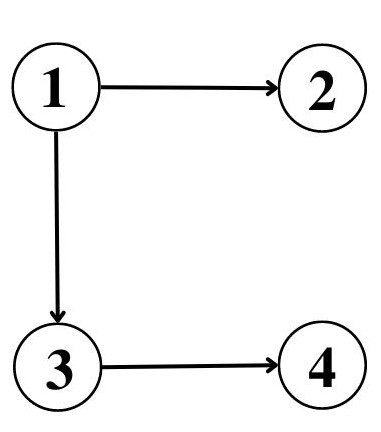
\includegraphics[scale=0.4]{Tema_2c_1.jpg}

Avem nodul 1 cu grad interior 0, deci îi vom adăuga restul de arce exterioare (spre nodurile cu care nu este adiacent).
Eliminăm nodul 1 din tabel și decrementăm gradul nodurilor care aveau muchie dinspre nodul 1.

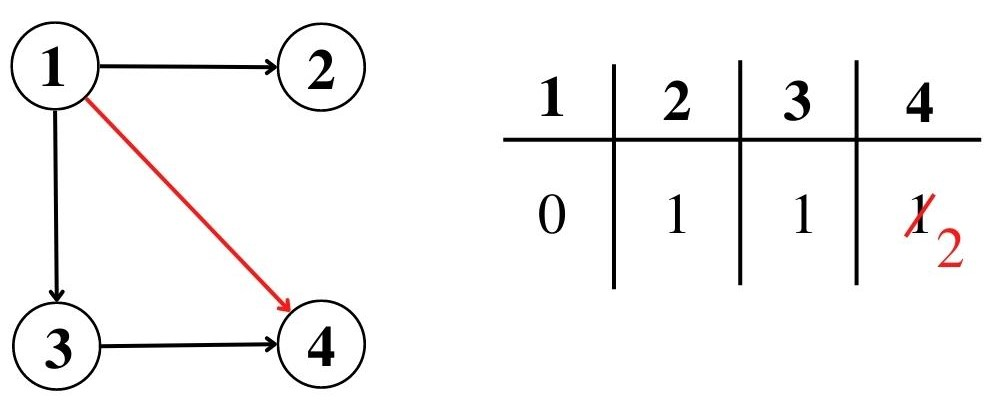
\includegraphics[scale=0.4]{Tema_2c_2.jpg}

I. Alegem nodul 2 cu grad interior 0, deci îi vom adăuga restul de arce exterioare (spre nodurile cu care nu este adiacent).
Eliminăm nodul 2 din tabel și decrementăm gradul nodurilor care aveau muchie dinspre nodul 2.

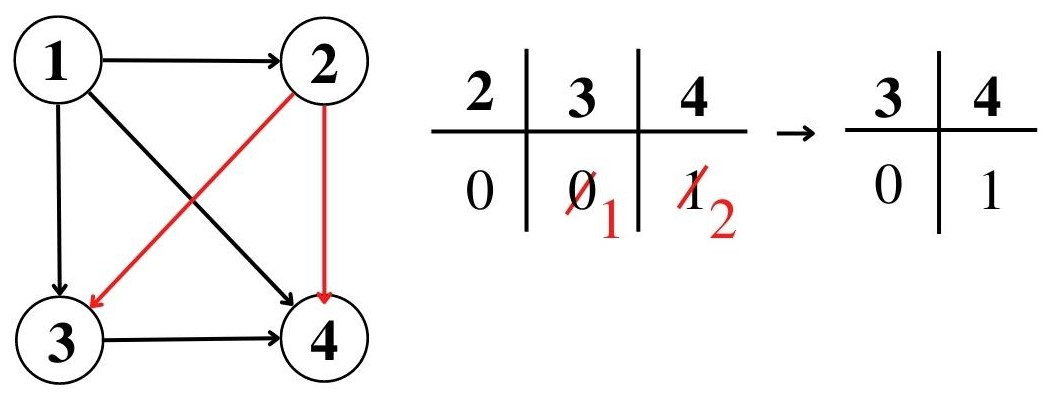
\includegraphics[scale=0.4]{Tema_2c_3.jpg}

II. Alegem nodul 3 cu grad interior 0, deci îi vom adăuga restul de arce exterioare (spre nodurile cu care nu este adiacent).
Eliminăm nodul 3 din tabel și decrementăm gradul nodurilor care aveau muchie dinspre nodul 3.

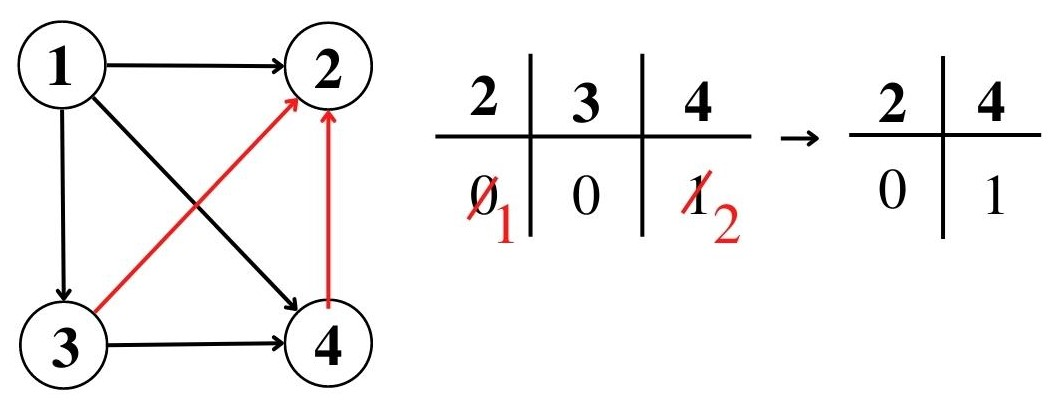
\includegraphics[scale=0.4]{Tema_2c_4.jpg}

Orice nod am alege dintre 2 si 3, digraful își va păstra proprietatea de aciclic.
    
    \item[d)]

Pentru a demonstra proprientatea P pentru orice graf G=(V,E), arătăm că putem să-l extindem pe $\vec{G'}$ la $\vec{K_n'}$ și pe $\vec{G''}$ la $\vec{K_n''}$ astfel încât orientările $\vec{K_n'}$ și $\vec{K_n''}$ să nu conțină cicluri (demonstrat la subpunctul punctul c).

    Putem obține orientarea aciclică $\vec{K_n''}$ din $\vec{K_n'}$ aplicând repetări succesive ale operației $reverse$ asupra arcelor din $\vec{K_n'}$ (conform subpunctului b).
    
    Eliminând arcele $E'= E(K_n \backslash E)$ din orientarea aciclică $\vec{K_n'}$ graful rezultat va avea în continuarea proprietatea de aciclicitate. În acest caz, proprietatea P este demonstrată pentru orice graf G.
    
\end{itemize}

\section{Exerci\c{t}iul 3}
 
\^{I}ncerc\u{a}m s\u{a} construim un contraexemplu pentru a demonstra incorectitudinea algoritmului sugerat de student. 

\^{I}n digraful G=(V,E) de mai jos costul drumului de la nodul X la nodul Z prin nodul Y este egal cu 3, în timp ce costul drumului prin nodurile W și U este egal cu 2. Având muchii de cost negativ nu putem aplica algoritmul lui Dijkstra, dar se observă c\u{a} drumul de cost minim de la X la Z este cel ce trece prin nodurile W și U.

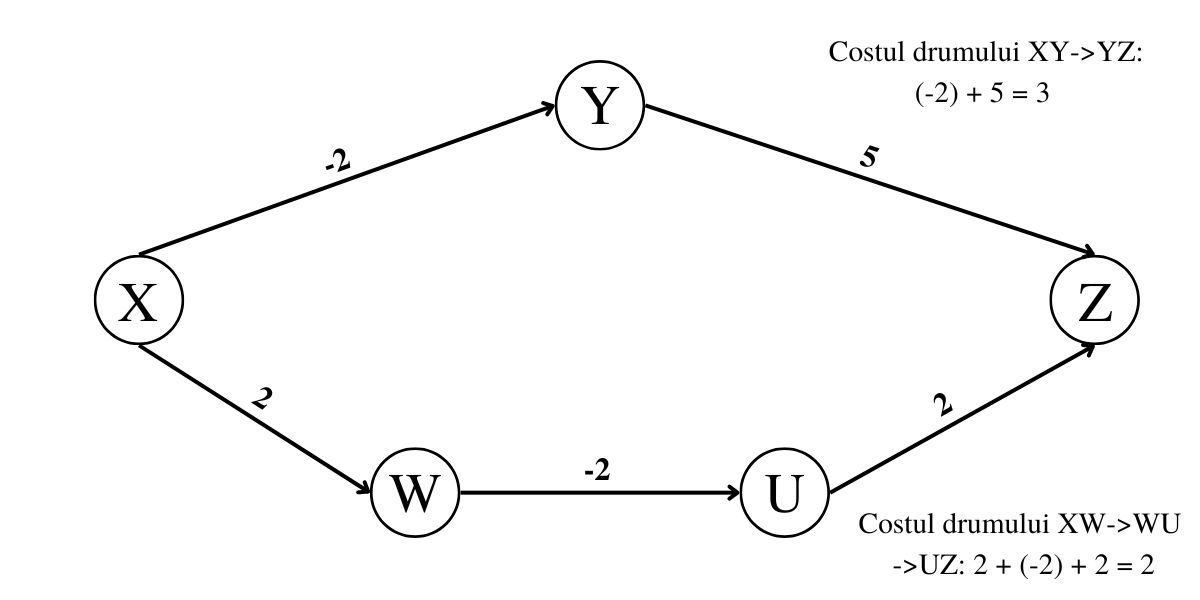
\includegraphics[scale=0.3]{313090941_827984621846159_5439754781801344054_n}

Alegem constanta k=2 astfel încât după adunarea acesteia la costul fiecărei muchii să nu mai existe muchii de cost negativ. Observăm că noul cost al drumului de la nodul X la nodul Z prin nodul Y este egal cu 7, în timp ce noul cost al drumului prin nodurile W și U este egal cu 8. Astfel se observă, aplicând algoritmul lui Dijkstra, că noul drum de cost minim de la X la Z este cel ce trece prin nodul Y.

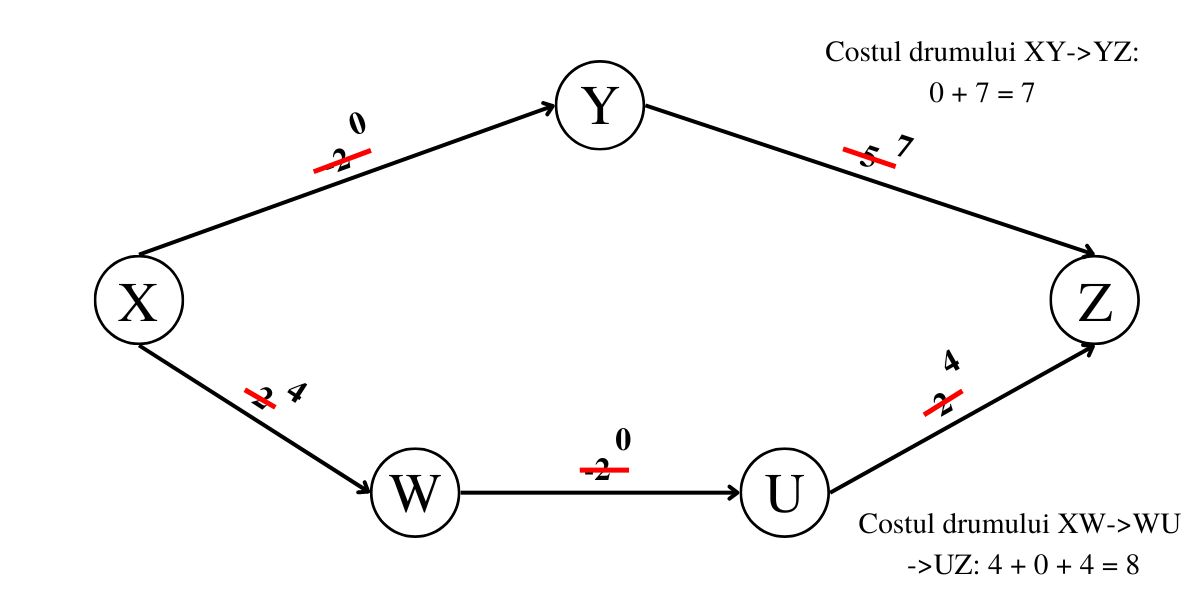
\includegraphics[scale=0.3]{307936481_3056475277977140_961538295951200335_n}

Se poate observa, uitându-ne la graful prezentat anterior, că la drumul de la nodul X la nodul Z prin nodul Y s-au adăugat două costante k=2 (acest drum fiind de lungime 2), iar la drumul de la nodul X la nodul Z prin nodurile W si U s-au adăugat trei costante k=2 (acest drum fiind de lungime 3). Astfel, se modifică drumul de cost minim.

În concluzie, algoritmul sugerat de student este incorect, fapt demonstrat prin contraxemplul de mai sus.

\section{Exerci\c{t}iul 4}

Algoritmul lui $Dijkstra$ poate rezolva problema P2 pe un digraf $\vec{G}$=(V,E) care are toate circuitele de cost pozitiv iar singurele posibile arce de cost negativ sunt cele care pleacă din sursa s$\in$V deoarece plecând cu cel mai mic cost posibil al unui arc din întreg digraful, costul total al circuitului nu va mai putea să scadă până la vizitarea ultimului nod din acest ciclu.

Având ca exemplu digraful $\vec{G}$=(V,E) desenat mai jos în care sursa s= \{ X \} și singurele arce de cost negativ sunt \{ XY \} =-1 și \{ XW \} =-3 putem trage următoarea concluzie: \\
Dacă am adăuga la arcul \{ XY \} și \{ XW \} o constantă k suficient de mare astfel încât ambele să devină pozitive, atunci am putea aplica algoritmul lui Dijkstra fără ca rezultatul să se schimbe deoarece adăugăm aceeași constantă o singura data la fiecare drum (spre deosebire de exercițiul al treilea în care adăugam un număr diferit de constante pentru fiecare drum, ceea ce schimba corectitudinea rezultatului).
    
	
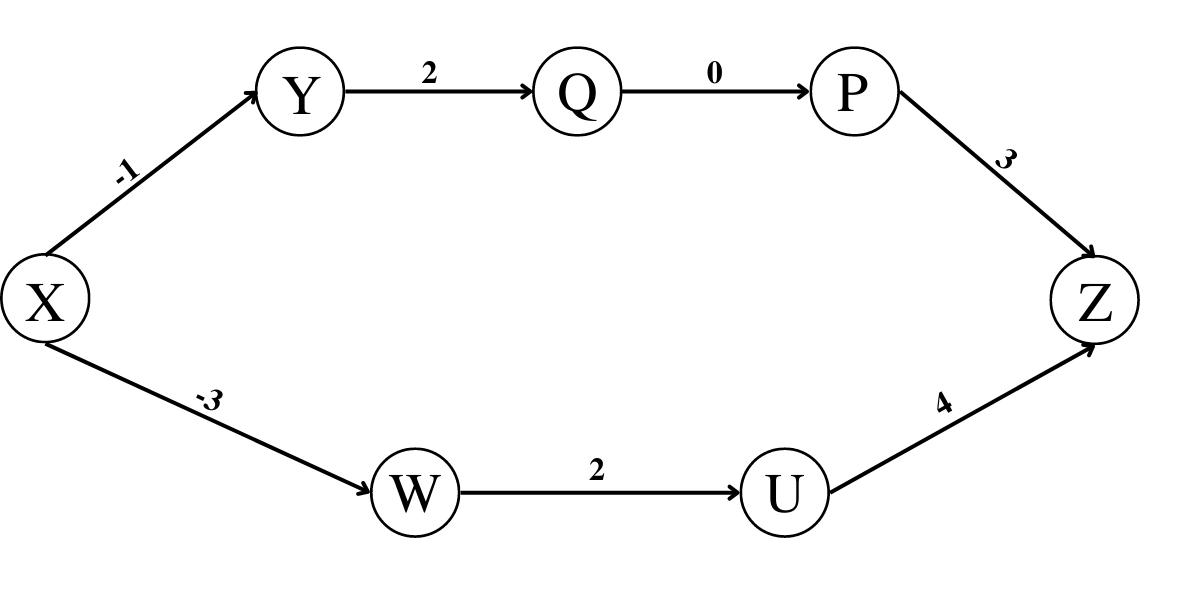
\includegraphics[scale=0.35]{Tema_4.jpg}
  


\end{document}
